\section*{Methods}

% =====================================================================
\subsection*{Cohort and labels}
% =====================================================================

\paragraph{TCGA-LUAD acquisition.}
We obtained $1{,}054$ FFPE-fixed haematoxylin-and-eosin (H\&E) WSIs
from $522$ LUAD patients in The Cancer Genome Atlas via the
GDC portal.\cite{tcga2014luad,gdc2024maf}
Diagnostic slides only (DX1--DX2) were retained; frozen, snap-frozen,
and resections without a paired primary diagnostic block were
excluded.
After quality filtering (Otsu tissue mask, pen-marker detector,
blur threshold; see \emph{Slide quality control} below) and after
exclusion of slides whose patient had no MAF mutation call for any
of the six target genes, $687$ analysable slides from $668$
patients remained.
Among them, $19$ patients had $\geq 2$ analysable slides; the
cross-validation was performed at the \emph{patient} level
(patient-stratified) to prevent leakage.

\paragraph{Target genes.}
Six driver mutations were retained on the basis of
LUAD-relevance and prevalence $\geq 5\%$ in the cohort
(\cref{tab:mutation_prevalence}):
\textit{TP53} (38.0\%), \textit{EGFR} (14.1\%), \textit{KRAS}
(28.5\%), \textit{STK11} (9.9\%), \textit{KEAP1} (14.3\%) and
\textit{RBM10} (5.4\%).

\begin{table}[h!]
\centering
% Table tab:mutation_prevalence — TCGA-LUAD cohort mutation prevalence
% (687 analysable diagnostic slides, 668 patients).
\small
\setlength{\tabcolsep}{8pt}
\begin{tabular}{l c c c}
\toprule
\textbf{Gene} & \textbf{Positive slides} ($n_{+}$) &
  \textbf{Prevalence} (\%) & \textbf{Conclusive verdict?} \\
\midrule
\textit{TP53}  & 261 & 38.0 & Yes \\
\textit{KRAS}  & 196 & 28.5 & No  \\
\textit{KEAP1} &  98 & 14.3 & No  \\
\textit{EGFR}  &  97 & 14.1 & Yes \\
\textit{STK11} &  68 &  9.9 & No  \\
\textit{RBM10} &  37 &  5.4 & No  \\
\bottomrule
\end{tabular}
\begin{flushleft}\footnotesize
$n_{+}\!=\!$~number of slides with at least one non-silent somatic
mutation called for the gene under the TCGA harmonised pipeline.
\emph{Conclusive verdict} is the cohort-level signal-presence flag
(mean AUROC $\geq\!0.70$ under five-fold cross-validation; see
Methods, Cross-validation and statistical analysis).
\end{flushleft}

\caption{Mutation prevalence in the analysable TCGA-LUAD cohort
($n\!=\!687$ slides from $668$ patients).
The Conclusive-verdict column anticipates the cohort-level outcome
of the five-fold cross-validation reported in Results.}
\label{tab:mutation_prevalence}
\end{table}
The corresponding mutation calls (MAF files) were obtained from
GDC and only non-silent variants retained: missense, nonsense,
frameshift, splice-site, in-frame insertion/deletion.
Synonymous and intronic variants were excluded.

\paragraph{Slide quality control.}
Each WSI was checked for: (i)~presence of a tissue area
$\geq 20\,\text{mm}^{2}$; (ii)~absence of large pen-marker
regions ($>10\%$ of the tissue area, detected by an HSV
band-pass); (iii)~per-tile blur (variance of the Laplacian)
above an empirically fixed threshold; (iv)~absence of large
histology artefacts (tears, folds, air bubbles).
Slides failing any criterion were excluded.

% =====================================================================
\subsection*{Tile extraction and tissue mask}
% =====================================================================

Each WSI was tiled at level~0 into non-overlapping
$224 \times 224$~px patches at $0.5~\mu\text{m}/\text{px}$
(approx.\ $20\times$).
A per-slide Otsu tissue mask discarded blank or background tiles
($<10\%$ tissue).
Per-tile pen-marker, blur and artefact checks were re-applied at
the tile level.
A 4-channel input ($\text{RGB}\,+\,\text{tissue-mask}$) was passed
to the encoder.\cite{wang2022ctranspath}

% =====================================================================
\subsection*{Pattern classifier (Artefact 1)}
% =====================================================================

The six-pattern classifier was trained on the Zenodo-ANORAK
dataset\cite{anorak2024,ANORAKZenodo}---$732$ expert-annotated
tiles spanning lepidic, acinar, papillary, micropapillary,
solid and cribriform, reduced to $637$ after exclusion of
``other tissue'' (class~0) tiles---using a \ctranspath{}
backbone\cite{wang2022ctranspath} and a fuzzy angular-margin head
(FuzzyArcLoss V2; full derivation and loss-family ablation
in\cite{limareina2026fuzzyarc}).
Per-sample fuzzy modulation of the ArcFace
margin\cite{deng2019arcface} is calibrated by Optuna
($s^{*}=46.1$, $m^{*}=0.518$, $\tau^{*}=0.448$,
$50$~trials, TPE sampler, MedianPruner).
Training protocol: AdamW (lr~$1\times10^{-4}$), cosine schedule
to $10^{-6}$, $5$-epoch warm-up, $120$ epochs, batch size $32$,
fp32; MixUp disabled.
Reported macro-F1 = $92.31\% \pm 2.04$ across 15 runs (5-fold $\times$
3 seeds) with $p = 0.001$ vs SphereFace and Cohen's $d = 1.00$.
Tile probabilities $\mathbf{p}\in\Delta^5$ become the pattern
channel used downstream.

% =====================================================================
\subsection*{MIL aggregation: PI-ABMIL and FC-MIL}
% =====================================================================

\paragraph{Tile representation.}
For each slide we retained the top $200$ tiles by encoder
embedding norm to keep the bag size constant.
Each tile contributed a $512$-d \ctranspath{} embedding
$\mathbf{e}\in\mathbb{R}^{512}$ and a $6$-d pattern probability
$\mathbf{p}\in\Delta^5$.
Six conditions were ablated as inputs:
B1 ($7$-d slide-level pattern fractions $\,+\,$ entropy
to XGBoost\cite{chen2016xgboost}); B2 ($512$-d embeddings only to
gated ABMIL\cite{ilse2018attention}); B3 ($6$-d pattern
probabilities only); PI-ABMIL ($512+6$ concat); A (one-hot of
$\arg\max\mathbf{p}$); FC-MIL ($512$-d embeddings to gated
attention $+$ $6$-d patterns to a fuzzy Choquet head).

\paragraph{PI-ABMIL.}
Gated attention\cite{ilse2018attention} computes
$\alpha_i = \softmax(\mathbf{v}^\top \tanh(\mathbf{W}_a
[\mathbf{e}_i;\mathbf{p}_i]) \odot \sigmoid(\mathbf{W}_b
[\mathbf{e}_i;\mathbf{p}_i]))$, and the slide representation is
$\mathbf{z} = \sum_i \alpha_i [\mathbf{e}_i;\mathbf{p}_i]$
followed by a linear gene head.
Hidden dim $128$, two-layer attention; $\approx 199{,}553$
parameters total.

\paragraph{FC-MIL (2-additive fuzzy Choquet).}
The slide-level pattern vector $\mathbf{P}\in\Delta^5$ is
aggregated by a differentiable
$2$-additive Choquet
integral~\cite{grabisch1996application,grabisch1997kapprox}.
A general fuzzy measure over $n\!=\!6$ patterns would require
$2^{n}\!-\!2\!=\!62$ parameters; the 2-additive approximation
reduces this to $6 + \binom{6}{2}\!=\!21$ parameters, fully
determined by singletons and pairs:
\begin{equation}
g(A) = \sum_{k\in A}\phi_k \;+\; \sum_{\{j,k\}\subseteq A} I_{jk},
\qquad A \subseteq \{1,\ldots,6\},
\label{eq:fuzzy_measure}
\end{equation}
where the singletons $\phi_k$ are Shapley
values~\cite{shapley1953value} (intrinsic contribution of pattern
$k$) and $I_{jk}$ are pairwise interaction indices
(positive $\Rightarrow$ synergy, negative $\Rightarrow$ redundancy).
We parameterise the singletons via a softmax
$\phi_k = e^{\psi_k}/\sum_l e^{\psi_l}$ on a learnable vector
$\psi\in\mathbb{R}^{6}$; the interactions are stored as a learnable
upper-triangular matrix with an $L_1$ sparsity prior
$\mathcal{R}_\text{int}=\lambda_I\sum_{j<k}|I_{jk}|$ and a soft
monotonicity penalty
$\mathcal{R}_\text{mono} =
\sum_{A\subseteq B}\max(0,\,g(A)\!-\!g(B))$
sampled by Monte Carlo at every batch.

For a slide-level fuzzy pattern probability vector
$\mathbf{P}\in\Delta^{5}$ sorted in ascending order
$P_{(1)}\!\leq\!P_{(2)}\!\leq\!\cdots\!\leq\!P_{(6)}$, the discrete
Choquet integral is
\begin{equation}
C_g(\mathbf{P}) \;=\; \sum_{k=1}^{6}
\bigl[P_{(k)}-P_{(k-1)}\bigr]\, g\!\left(A_{(k)}\right),
\quad A_{(k)} \!=\! \{(k),\ldots,(6)\},
\label{eq:choquet_integral}
\end{equation}
with $P_{(0)}\!:=\!0$.
The output $\mathbf{c}_s\in\mathbb{R}^{6}$ is concatenated with the
gated-attention embedding $\mathbf{z}_\mathrm{attn}\in\mathbb{R}^{256}$
and projected to the per-gene prediction.
\fcmil{} is the architectural primitive that exposes
pattern--pattern interactions as the $15$ scalars $I_{jk}$ for
direct clinical inspection at inference time.

% =====================================================================
\subsection*{Cross-validation and statistical analysis}
% =====================================================================

Five-fold patient-stratified cross-validation; folds were
created with mutation-stratified shuffling at the patient level to
preserve gene prevalence.
Per-fold metrics: \auroc{} (primary, prevalence-invariant),
\auprc{}\cite{davis2006auprc} (secondary, prevalence-sensitive),
positive class operating thresholds via Youden's
$J$.\cite{youden1950index}

\paragraph{Conclusive verdict criterion.}
The cohort-level Conclusive/Inconclusive flag
(\cref{tab:viz_folds_methods}) is defined as
\begin{equation}
\mathrm{Conclusive}(\mathrm{gene}) \iff
\frac{1}{5}\sum_{f=1}^{5}\auroc_{f}^{(\mathrm{gene})} \;\geq\; 0.70,
\label{eq:conclusive_verdict}
\end{equation}
where $\auroc_f^{(\mathrm{gene})}$ is the held-out AUROC of fold $f$
under the best MIL aggregator for that gene.
This is a population-level signal-presence flag, \emph{not} a
per-slide confidence threshold; the per-slide $P$-value (the
softmax-normalised mutation probability of the gene-specific head)
is reported independently and inherits the calibration of the
underlying \piabmil{} or \fcmil{} classifier.

\begin{table}[h!]
\centering
% Table tab:viz_folds_methods — Conclusive / Inconclusive verdict bands
% over the five-fold patient-stratified CV protocol.
% Wide table (4 cols, last col long): use tabularx so the "Genes" column
% wraps cleanly inside the text width.
\small
\setlength{\tabcolsep}{6pt}
\begin{tabularx}{\linewidth}{l c c X}
\toprule
\textbf{Verdict} & \textbf{Mean AUROC band} &
  \makecell{\textbf{Per-slide score}\\\textbf{still reported?}} &
  \textbf{Genes (this cohort)} \\
\midrule
Conclusive   & $\geq 0.70$ & Yes &
  \textit{TP53} ($0.717$), \textit{EGFR} ($0.701$)$^{\dagger}$ \\
Inconclusive & $< 0.70$    & Yes &
  \textit{KRAS} ($0.609$), \textit{STK11} ($0.695$)$^{\dagger}$,
  \textit{KEAP1} ($0.610$), \textit{RBM10} ($0.661$) \\
\bottomrule
\end{tabularx}
\begin{flushleft}\footnotesize
The verdict is a population-level signal-presence flag, not a
per-slide confidence threshold; the per-slide model probability is
reported independently in every case.
$^{\dagger}$EGFR and STK11 are within $\pm 0.01$ of the threshold
under the upper-tier conditions and are reported here under their
best-tier AUROC. The Conclusive/Inconclusive flag is robust to
choice of MIL aggregator within the upper tier; the per-gene
ranking is not.
\end{flushleft}

\caption{Conclusive/Inconclusive verdict bands and their assignment
to the six target genes under the five-fold patient-stratified CV
protocol used throughout the paper.}
\label{tab:viz_folds_methods}
\end{table}

% =====================================================================
\subsection*{Six-level interpretability stack}
% =====================================================================

\textbf{(L1) ABMIL attention overlay:} the $\alpha_i$ weights are
rendered as a heat-map on the slide thumbnail.
\textbf{(L2) Pattern overlay:} per-tile $\arg\max\mathbf{p}$
rendered as a discrete colour layer; each tile is hover-clickable.
\textbf{(L3) SHAP:}
TreeSHAP\cite{lundberg2017shap,lundberg2020treeshap} for B1;
DeepSHAP for the MIL conditions; the slide-level SHAP value is
decomposed into the embedding-channel and pattern-channel
contributions.
\textbf{(L4) Choquet--Shapley and pairwise
interactions:}\cite{shapley1953value,grabisch1996application}
the FC-MIL parameter set is read out per slide.
\textbf{(L5) Per-slide channel ablation:} the prediction is
recomputed with each input channel zeroed; the resulting
$\Delta\auroc$ table is reported.
\textbf{(L6) Fuzzy linguistic labels:} continuous scores
$x\!\in\![0,1]$ (per-slide $P$-value, Shapley values
$\phi_k$, interaction magnitudes $|I_{jk}|$) are mapped to one of
five linguistic categories
$\{\mathrm{VL},\mathrm{L},\mathrm{M},\mathrm{H},\mathrm{VH}\}$ via
the trapezoidal membership functions
\begin{equation}
\mu_{\mathrm{cat}}(x;\,a,b,c,d) =
\max\!\left(0,\;
\min\!\left(1,\,\frac{x-a}{b-a},\,\frac{d-x}{d-c}\right)\right),
\label{eq:trap_mf}
\end{equation}
with breakpoints calibrated against the SOLCA-CISOL pilot reader
study so that the categorical word is the one the on-call
pathologist would have used at the same score range
($\mathrm{VL}\!:\![0,0.10]$, $\mathrm{L}\!:\![0.10,0.30]$,
$\mathrm{M}\!:\![0.30,0.70]$, $\mathrm{H}\!:\![0.70,0.90]$,
$\mathrm{VH}\!:\![0.90,1.00]$; overlap of $0.10$ between adjacent
trapezoids).
The LLM agent below is permitted to use only these categorical
words when stating evidence strength, removing spurious decimal
precision and monotonic claims on probabilities inside the
\emph{Moderate} band.

% =====================================================================
\subsection*{LLM explanation layer with dual anti-hallucination}
% =====================================================================

Each slide-level evidence bundle (gene, P-value, L1--L6 outputs,
Conclusive flag, similar curated cases) is rendered as a structured
JSON document and passed to a prompt-engineered LLM agent
(provider-agnostic; we validated with GPT-4 and Claude Sonnet).
The agent is instructed:
\textit{(a)} to use only the fuzzy linguistic labels of
\cref{eq:trap_mf} for probabilities (constraining \emph{how} it
speaks);
\textit{(b)} to invoke only entities/edges present in the
three-layer knowledge graph $\mathcal{K} = (V, E)$ depicted in
\cref{fig:kg_three_layers}, built from
NCIt~\cite{sioutos2007ncit} (concept layer $V_C$),
MONDO~\cite{mondo_shefchek2020} (disease layer $V_D$) and a
dynamic per-case DeepSearch literature layer $V_L$ with PMID
provenance attached to every $e\in E$
(constraining \emph{what} it can claim);
\textit{(c)} to surface any deactivated edges as
``previously hypothesised, now contested'' rather than deleting
them, preserving full auditability.

\begin{figure}[h!]
  \centering
  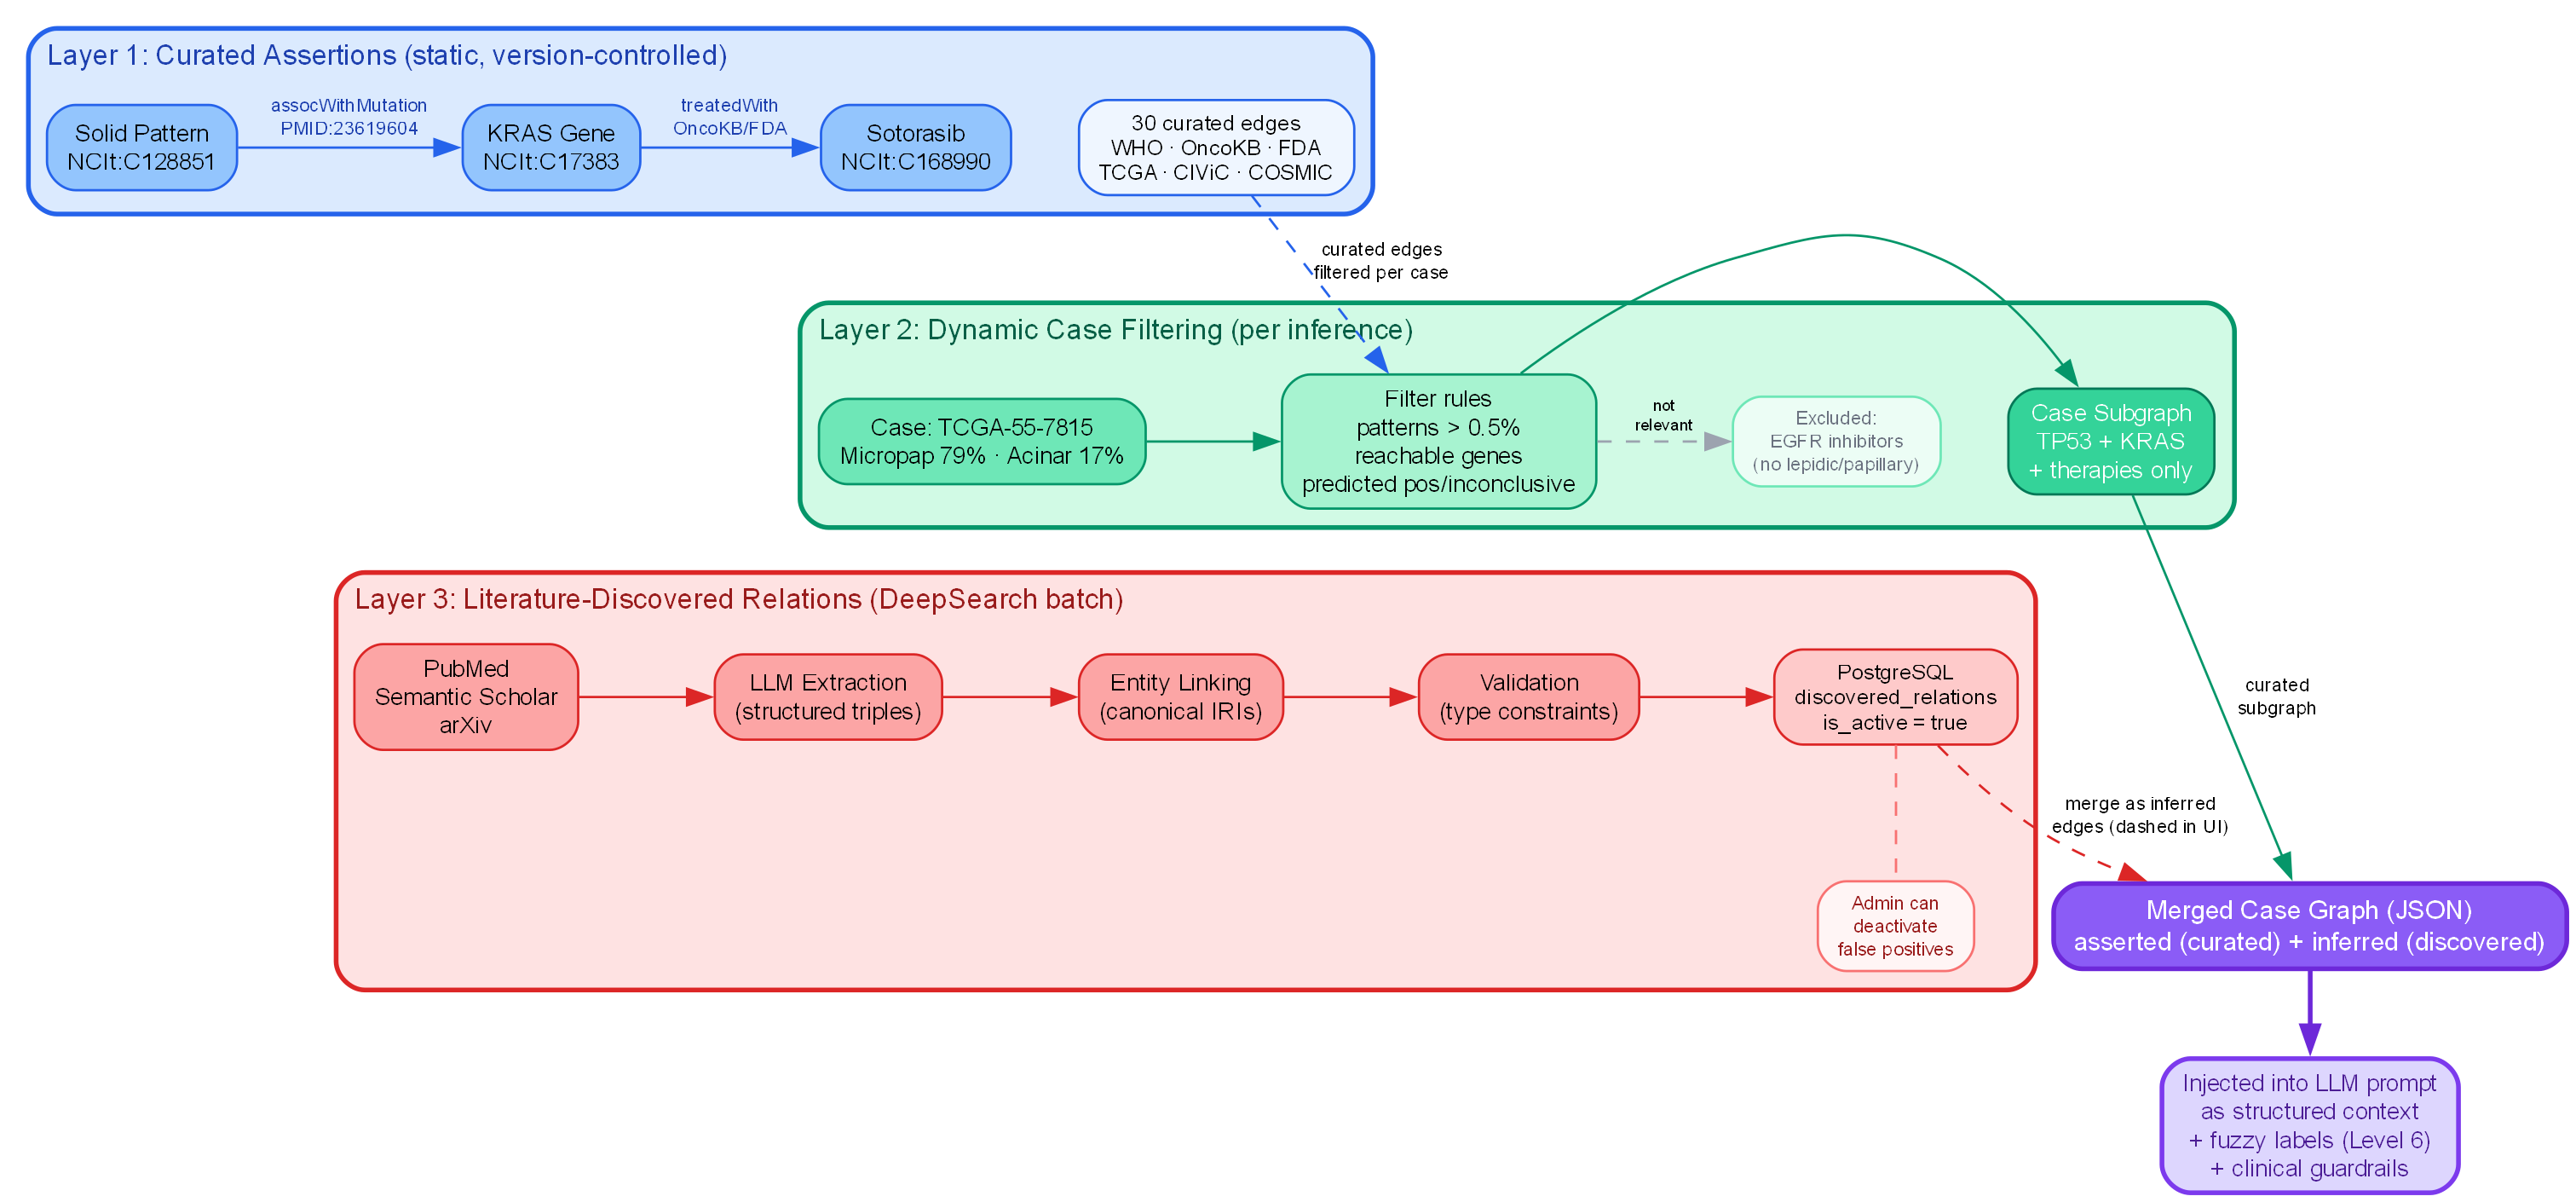
\includegraphics[width=\linewidth]{kg_three_layers_method}
  \caption{\textbf{Three-layer knowledge graph
  $\mathcal{K} = (V_C \cup V_D \cup V_L,\, E)$ used to ground the
  LLM explanation layer.}
  $V_C$: NCIt~\cite{sioutos2007ncit} concept nodes (genes,
  pathways, histological patterns).
  $V_D$: MONDO~\cite{mondo_shefchek2020} disease nodes
  (e.g.\ \emph{lung adenocarcinoma},
  \emph{invasive mucinous adenocarcinoma}).
  $V_L$: a per-case dynamic literature layer built by DeepSearch
  at query time, each node carrying a PMID provenance tag that is
  exposed to the user as a click-through citation.
  The agent's prompt grammar permits it to invoke only entities
  and edges in $V$ and $E$; this constrains \emph{what} the
  narrative can claim. \cref{eq:trap_mf} constrains \emph{how}
  evidence strength is verbalised.}
  \label{fig:kg_three_layers}
\end{figure}

% =====================================================================
\subsection*{Reproducibility, data and code availability}
% =====================================================================

All experiments were run on a single H100 GPU (training) and
a T4 GPU (inference; live LCHAI deployment at
\url{https://lchai.gptfy.biz}).
PyTorch 2.x, CTransPath checkpoint as published.\cite{wang2022ctranspath}
Seeds: 42, 123, 2026.
Source code: \url{https://github.com/slima2/lchai}.
TCGA-LUAD data: \url{https://portal.gdc.cancer.gov}.
ANORAK Zenodo dataset: \cite{ANORAKZenodo}.
Mutation calls (MAF): GDC, accessed 03~April~2026.

% =====================================================================
\subsection*{Ethical approval}
% =====================================================================

The TCGA-LUAD cohort is a publicly available, de-identified
research dataset published under the controlled-access policy of
the NIH Genomic Data Commons.\cite{tcga2014luad}
The SOLCA-CISOL pilot validation study was approved by the
Comit\'e de \'Etica de Investigaci\'on en Seres Humanos
(CEISH) of SOLCA Ecuador (approval 2026-014).

